\documentclass[tikz,border=0pt]{standalone}
\usepackage{xcolor}
\usetikzlibrary{calc}
% Palette: Sam_Comm_final.png by eye, and the drones and raiders.
\definecolor{ink}{HTML}{3B2340}
\definecolor{sky}{HTML}{EFC46A}
\definecolor{skyhi}{HTML}{F5DA92}
\definecolor{skylow}{HTML}{E9B060}
\definecolor{cloud}{HTML}{F2D58A}
\definecolor{paper}{HTML}{FBEFD0}
\definecolor{cream}{HTML}{FFF6E0}
\definecolor{white}{HTML}{FFFFFF}
\definecolor{wallA}{HTML}{E88A73}
\definecolor{wallB}{HTML}{EE9F7E}
\definecolor{wallC}{HTML}{E47A7E}
\definecolor{wallD}{HTML}{F0B07E}
\definecolor{wallE}{HTML}{D9765F}
\definecolor{wallF}{HTML}{E99A8A}
\definecolor{greenA}{HTML}{8DBB7E}
\definecolor{greenB}{HTML}{6FA77A}
\definecolor{greenC}{HTML}{A9C97F}
\definecolor{greenD}{HTML}{5E9C6A}
\definecolor{greenE}{HTML}{4A8060}
\definecolor{sage}{HTML}{9DB98A}
\definecolor{sagedark}{HTML}{6F8F66}
\definecolor{sagelight}{HTML}{C2D6A6}
\definecolor{window}{HTML}{F6E7A0}
\definecolor{windark}{HTML}{8C5A64}
\definecolor{metal}{HTML}{8D9A93}
\definecolor{metaldark}{HTML}{5E6B66}
\definecolor{metallight}{HTML}{B9C4BC}
\definecolor{wood}{HTML}{B9835A}
\definecolor{wooddark}{HTML}{8C5A3C}
\definecolor{woodlight}{HTML}{D9A66F}
\definecolor{stone}{HTML}{E7C9A0}
\definecolor{stonedark}{HTML}{C9A47E}
\definecolor{concrete}{HTML}{D8C3A4}
\definecolor{concretedark}{HTML}{B8A084}
\definecolor{asphalt}{HTML}{8E7A86}
\definecolor{asphaltdark}{HTML}{6E5C68}
\definecolor{roadline}{HTML}{F6E7A0}
\definecolor{kerb}{HTML}{D8B48C}
\definecolor{red}{HTML}{E0483E}
\definecolor{redlight}{HTML}{F27A6A}
\definecolor{gold}{HTML}{FFB000}
\definecolor{goldlight}{HTML}{FFD54F}
\definecolor{teal}{HTML}{4FA3A0}
\definecolor{tealdark}{HTML}{3C8582}
\definecolor{magenta}{HTML}{FF2E88}
\definecolor{cyan}{HTML}{13CFE3}
\definecolor{violet}{HTML}{8A5BD6}
\definecolor{orange}{HTML}{F2803A}
\definecolor{pink}{HTML}{F48FB1}
\definecolor{glow}{HTML}{4FE6E0}
\definecolor{glowhi}{HTML}{C8FFF9}
\definecolor{hot}{HTML}{FF6A1A}
\definecolor{hothi}{HTML}{FFD07A}
\definecolor{armour}{HTML}{7E7A86}
\definecolor{armourdark}{HTML}{5A5466}
\definecolor{armourlight}{HTML}{A8A2B0}
\definecolor{wasp}{HTML}{E0A82E}
\definecolor{waspdark}{HTML}{B07E1A}
\definecolor{moth}{HTML}{F2E6C8}
\definecolor{mothdark}{HTML}{D2C09A}
\definecolor{hornet}{HTML}{3C8582}
\definecolor{hornetdark}{HTML}{2C6260}
\definecolor{warden}{HTML}{E47A7E}
\definecolor{wardendark}{HTML}{B85A62}
\definecolor{tick}{HTML}{8DBB7E}
\definecolor{tickdark}{HTML}{5E8A5A}
\definecolor{strider}{HTML}{D9765F}
\definecolor{striderdark}{HTML}{A8543F}
\definecolor{jacket}{HTML}{6FA77A}
\definecolor{jacketb}{HTML}{4FA3A0}
\definecolor{jacketc}{HTML}{E88A73}
\definecolor{jacketd}{HTML}{F0B07E}
\definecolor{skin}{HTML}{F2C49A}
\definecolor{skinb}{HTML}{C98C6A}
\definecolor{skinc}{HTML}{8C5A3C}
\definecolor{hair}{HTML}{3B2340}
\definecolor{goo}{HTML}{B6E35A}
\definecolor{goodark}{HTML}{7FB23A}
\newcommand{\Ink}{1.8pt}
\tikzset{inked/.style={draw=ink, line width=\Ink, line join=round, line cap=round}}
\begin{document}
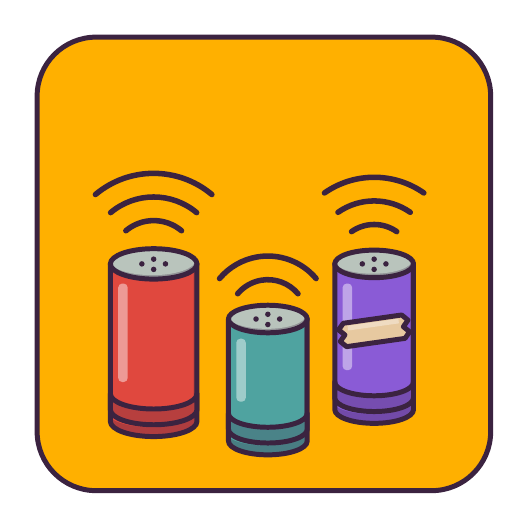
\begin{tikzpicture}
\clip (0,0) rectangle (6,6);
\fill[gold] [rounded corners=0.75cm] (0.12,0.12) rectangle (5.88,5.88);
\begin{scope}\clip [rounded corners=0.75cm] (0.12,0.12) rectangle (5.88,5.88);
\begin{scope}[shift={(1.6,1)}, rotate=0, xscale=1, yscale=1]
\begin{scope}\clip (-0.55,2) -- (-0.55,0) arc[start angle=180, end angle=360, x radius=0.55, y radius=0.193] -- (0.55,2) -- cycle;
\fill[red!70!ink] (-0.55,2) -- (-0.55,0) arc[start angle=180, end angle=360, x radius=0.55, y radius=0.193] -- (0.55,2) -- cycle;
\fill[red, shift={(-0.042,0.12)}] (-0.55,2) -- (-0.55,0) arc[start angle=180, end angle=360, x radius=0.55, y radius=0.193] -- (0.55,2) -- cycle;
\end{scope}
\draw[inked] (-0.55,2) -- (-0.55,0) arc[start angle=180, end angle=360, x radius=0.55, y radius=0.193] -- (0.55,2) -- cycle;
\begin{scope}\clip (-0.55,0.35) -- (-0.55,0.15) arc[start angle=180, end angle=360, x radius=0.55, y radius=0.193] -- (0.55,0.35) arc[start angle=0, end angle=-180, x radius=0.55, y radius=0.193] -- cycle;
\fill[red!75!ink!70!ink] (-0.55,0.35) -- (-0.55,0.15) arc[start angle=180, end angle=360, x radius=0.55, y radius=0.193] -- (0.55,0.35) arc[start angle=0, end angle=-180, x radius=0.55, y radius=0.193] -- cycle;
\fill[red!75!ink, shift={(0,0)}] (-0.55,0.35) -- (-0.55,0.15) arc[start angle=180, end angle=360, x radius=0.55, y radius=0.193] -- (0.55,0.35) arc[start angle=0, end angle=-180, x radius=0.55, y radius=0.193] -- cycle;
\end{scope}
\draw[inked] (-0.55,0.35) -- (-0.55,0.15) arc[start angle=180, end angle=360, x radius=0.55, y radius=0.193] -- (0.55,0.35) arc[start angle=0, end angle=-180, x radius=0.55, y radius=0.193] -- cycle;
\begin{scope}\clip (0,2) ellipse (0.55 and 0.193);
\fill[metallight!70!ink] (0,2) ellipse (0.55 and 0.193);
\fill[metallight, shift={(-0.017,0.05)}] (0,2) ellipse (0.55 and 0.193);
\end{scope}
\draw[inked] (0,2) ellipse (0.55 and 0.193);
\fill[ink] (-0.15,2) circle (0.035);
\fill[ink] (0,2.06) circle (0.035);
\fill[ink] (0.15,2) circle (0.035);
\fill[ink] (0,1.93) circle (0.035);
\fill[white, opacity=0.45, rounded corners=0.05cm] (-0.45,0.5) rectangle (-0.33,1.75);
\end{scope}
\begin{scope}[shift={(3.05,0.75)}, rotate=0, xscale=1, yscale=1]
\begin{scope}\clip (-0.5,1.55) -- (-0.5,0) arc[start angle=180, end angle=360, x radius=0.5, y radius=0.175] -- (0.5,1.55) -- cycle;
\fill[teal!70!ink] (-0.5,1.55) -- (-0.5,0) arc[start angle=180, end angle=360, x radius=0.5, y radius=0.175] -- (0.5,1.55) -- cycle;
\fill[teal, shift={(-0.042,0.12)}] (-0.5,1.55) -- (-0.5,0) arc[start angle=180, end angle=360, x radius=0.5, y radius=0.175] -- (0.5,1.55) -- cycle;
\end{scope}
\draw[inked] (-0.5,1.55) -- (-0.5,0) arc[start angle=180, end angle=360, x radius=0.5, y radius=0.175] -- (0.5,1.55) -- cycle;
\begin{scope}\clip (-0.5,0.35) -- (-0.5,0.15) arc[start angle=180, end angle=360, x radius=0.5, y radius=0.175] -- (0.5,0.35) arc[start angle=0, end angle=-180, x radius=0.5, y radius=0.175] -- cycle;
\fill[teal!75!ink!70!ink] (-0.5,0.35) -- (-0.5,0.15) arc[start angle=180, end angle=360, x radius=0.5, y radius=0.175] -- (0.5,0.35) arc[start angle=0, end angle=-180, x radius=0.5, y radius=0.175] -- cycle;
\fill[teal!75!ink, shift={(0,0)}] (-0.5,0.35) -- (-0.5,0.15) arc[start angle=180, end angle=360, x radius=0.5, y radius=0.175] -- (0.5,0.35) arc[start angle=0, end angle=-180, x radius=0.5, y radius=0.175] -- cycle;
\end{scope}
\draw[inked] (-0.5,0.35) -- (-0.5,0.15) arc[start angle=180, end angle=360, x radius=0.5, y radius=0.175] -- (0.5,0.35) arc[start angle=0, end angle=-180, x radius=0.5, y radius=0.175] -- cycle;
\begin{scope}\clip (0,1.55) ellipse (0.5 and 0.175);
\fill[metallight!70!ink] (0,1.55) ellipse (0.5 and 0.175);
\fill[metallight, shift={(-0.017,0.05)}] (0,1.55) ellipse (0.5 and 0.175);
\end{scope}
\draw[inked] (0,1.55) ellipse (0.5 and 0.175);
\fill[ink] (-0.15,1.55) circle (0.035);
\fill[ink] (0,1.61) circle (0.035);
\fill[ink] (0.15,1.55) circle (0.035);
\fill[ink] (0,1.48) circle (0.035);
\fill[white, opacity=0.45, rounded corners=0.05cm] (-0.4,0.5) rectangle (-0.28,1.3);
\end{scope}
\begin{scope}[shift={(4.4,1.15)}, rotate=0, xscale=1, yscale=1]
\begin{scope}\clip (-0.5,1.85) -- (-0.5,0) arc[start angle=180, end angle=360, x radius=0.5, y radius=0.175] -- (0.5,1.85) -- cycle;
\fill[violet!70!ink] (-0.5,1.85) -- (-0.5,0) arc[start angle=180, end angle=360, x radius=0.5, y radius=0.175] -- (0.5,1.85) -- cycle;
\fill[violet, shift={(-0.042,0.12)}] (-0.5,1.85) -- (-0.5,0) arc[start angle=180, end angle=360, x radius=0.5, y radius=0.175] -- (0.5,1.85) -- cycle;
\end{scope}
\draw[inked] (-0.5,1.85) -- (-0.5,0) arc[start angle=180, end angle=360, x radius=0.5, y radius=0.175] -- (0.5,1.85) -- cycle;
\begin{scope}\clip (-0.5,0.35) -- (-0.5,0.15) arc[start angle=180, end angle=360, x radius=0.5, y radius=0.175] -- (0.5,0.35) arc[start angle=0, end angle=-180, x radius=0.5, y radius=0.175] -- cycle;
\fill[violet!75!ink!70!ink] (-0.5,0.35) -- (-0.5,0.15) arc[start angle=180, end angle=360, x radius=0.5, y radius=0.175] -- (0.5,0.35) arc[start angle=0, end angle=-180, x radius=0.5, y radius=0.175] -- cycle;
\fill[violet!75!ink, shift={(0,0)}] (-0.5,0.35) -- (-0.5,0.15) arc[start angle=180, end angle=360, x radius=0.5, y radius=0.175] -- (0.5,0.35) arc[start angle=0, end angle=-180, x radius=0.5, y radius=0.175] -- cycle;
\end{scope}
\draw[inked] (-0.5,0.35) -- (-0.5,0.15) arc[start angle=180, end angle=360, x radius=0.5, y radius=0.175] -- (0.5,0.35) arc[start angle=0, end angle=-180, x radius=0.5, y radius=0.175] -- cycle;
\begin{scope}\clip (0,1.85) ellipse (0.5 and 0.175);
\fill[metallight!70!ink] (0,1.85) ellipse (0.5 and 0.175);
\fill[metallight, shift={(-0.017,0.05)}] (0,1.85) ellipse (0.5 and 0.175);
\end{scope}
\draw[inked] (0,1.85) ellipse (0.5 and 0.175);
\fill[ink] (-0.15,1.85) circle (0.035);
\fill[ink] (0,1.91) circle (0.035);
\fill[ink] (0.15,1.85) circle (0.035);
\fill[ink] (0,1.78) circle (0.035);
\fill[white, opacity=0.45, rounded corners=0.05cm] (-0.4,0.5) rectangle (-0.28,1.6);
\filldraw[inked,fill=stone] (-0.35,0.799) -- (0.392,0.904) -- (0.451,0.988) -- (0.371,1.052) -- (0.43,1.136) -- (0.35,1.201) -- (-0.392,1.096) -- (-0.451,1.012) -- (-0.371,0.948) -- (-0.43,0.864) -- cycle;
\fill[white, opacity=0.35] (-0.329,1.004) -- (0.315,1.095) -- (0.307,1.154) -- (-0.337,1.064) -- cycle;
\end{scope}
% emblem: sound arcs
\draw[ink, line width=2pt, line cap=round] (1.954,3.421) arc[start angle=50, end angle=130, radius=0.55];
\draw[ink, line width=2pt, line cap=round] (2.146,3.651) arc[start angle=50, end angle=130, radius=0.85];
\draw[ink, line width=2pt, line cap=round] (2.339,3.881) arc[start angle=50, end angle=130, radius=1.15];
% emblem: sound arcs
\draw[ink, line width=2pt, line cap=round] (3.433,2.621) arc[start angle=40, end angle=140, radius=0.5];
\draw[ink, line width=2pt, line cap=round] (3.663,2.814) arc[start angle=40, end angle=140, radius=0.8];
% emblem: sound arcs
\draw[ink, line width=2pt, line cap=round] (4.687,3.41) arc[start angle=55, end angle=125, radius=0.5];
\draw[ink, line width=2pt, line cap=round] (4.859,3.655) arc[start angle=55, end angle=125, radius=0.8];
\draw[ink, line width=2pt, line cap=round] (5.031,3.901) arc[start angle=55, end angle=125, radius=1.1];
\end{scope}
\draw[inked] [rounded corners=0.75cm] (0.12,0.12) rectangle (5.88,5.88);
\end{tikzpicture}
\end{document}
